\chapter{Proposal of Tool Refactoring}%
\label{chapt-proposta}

While working and utilizing the RMT toll, many flaws were found and described on \cref{subsub-limitation}. A new internal and external architecture was proposed focusing on solving those problems; these modifications will allow the system to scale better, provide better performance and make it easy to use by accessing the tool by the cloud.

The \cref{sec-cloud} explain the cloud solution of the new RMT architecture; \cref{sub-async} talks about the ways to apply asynchronous operations to the tool; \cref{sub-tests} explaining about applying tests on the RMT; \cref{sec-closingproposal} comments about the closing remarks


\section{Architecture Refactoring \& Cloud Approach}
\label{sec-cloud}
The new architecture has a few changes in the communication over the services. There are three services, and the metrics service calculates the metrics. The detection service is used to find the patterns, and the intermediary service is used to communicate with all the services and clients, as shown in \Cref{fig-architecture}.

The services will be the same, changing the communication type to queues over HTTP requests. The change is mainly to create a communication with more configuration over failure, as the service must acknowledge the message, or it will return to the queue. When using horizontal escalation, other service instances can consume it. On the HTTP request, the retry has to be implemented on the client side according to the server response. This responsibility does not exist using a queue adequately configured.

The changes are focused on improving the speed and usability of the tool; with that in mind, the infrastructure will be deployed on the AWS cloud, and the technologies used are available to be used locally with the AWS LocalStack, so if anyone wants to deploy the tool locally it's going to be possible with no trouble.

\begin{figure}[ht!]
\SetCaptionWidth{\textwidth}
\caption{RMT new architecture diagram}
\label{fig-async}
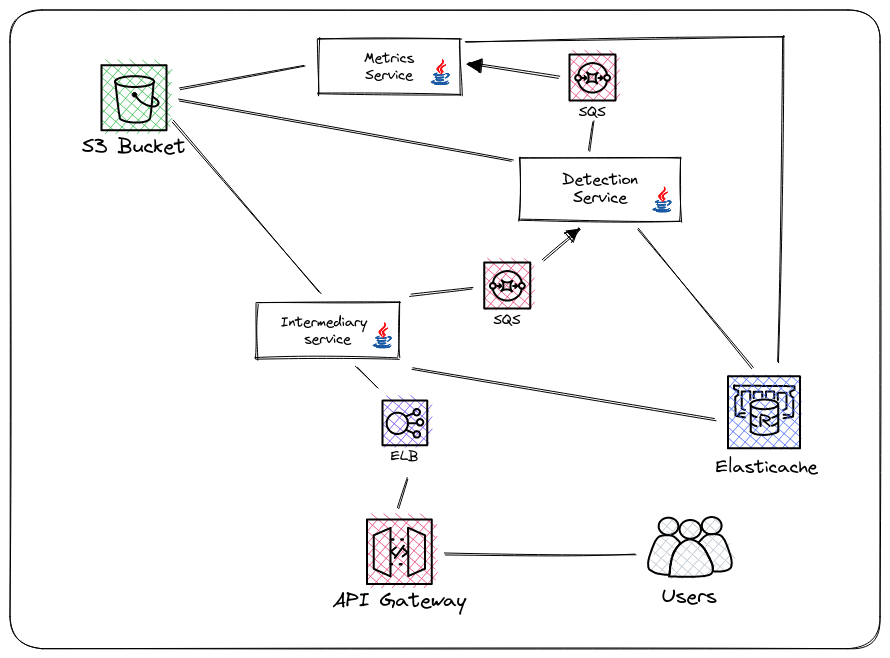
\includegraphics[width =\textwidth, scale=0.2]{Chapter-4/Figures/Async.png}
\SourceOrNote{Own authorship (2023)}
\end{figure}

In \Cref{fig-async}, the representation is made using AWS services. The services used are Fargate, Amazon SQS, AWS API gateway, ELB, Elasticache Redis, and S3 Bucket.
\begin{itemize}
\item Fargate: is a container manager from AWS. It was chosen because all the services will be converted to run-over docker containers, so they can be pre-configured with a DockerFile making the deployment and scalability faster, and it will have the same configuration for every instance to scale horizontally.
\item Amazon SQS: is a fully managed queue service provided by AWS.
\item Elasticache Redis: is a fully managed cache service with Redis, a fast and reliable memory database.
\item S3 Bucket:  is a fully managed file storage.
\item ELB: is an elastic load balancer fully managed by AWS.
\item API gateway: is a layer of communication to access endpoints through the internet to the AWS.
\end{itemize}


The new architecture works quite differently from the old one, starting with the database; the RMT was supposed to save the files over MongoDB, which offers the GridFs to save files over the database; on the renewal, this database was substituted by two services, the Amazon S3 and the Elasticache. The S3 will store all the files as it is the only focus of the tool, differing from the MongoDB. Elasticache is a cache service that fits perfectly to store project information. It provides fast reads and writes as it writes over memory and not disk; it will be configured with a time to live of one day because storing project information for long periods is unnecessary.

The SQS will substitute most of the REST calls of the tools and change how it works; on the old architecture, the Intermediary service works as a load balancer, service registry, which the ELB substituted, and back end for frontend (BFF). In the new architecture, the intermediary service will work only as a BFF communicating with the Detection service. It will communicate with the metrics service independently, as it already knows if a refactoring candidate exists. That direct communication will remove the point of failure because, in the old architecture, the detection service answers for the intermediary service, which sends the return to the client. The client starts the detection service by a REST call relying on the client connection.

As the architecture works asynchronously, the client will have to pull for the information on the BFF, verify the status on the Elasticache, and send the information to the client if it's ready.

\begin{figure}[ht!]
\SetCaptionWidth{\textwidth}
\caption{New Architecture Use Case}
\label{fig-usecasenew}
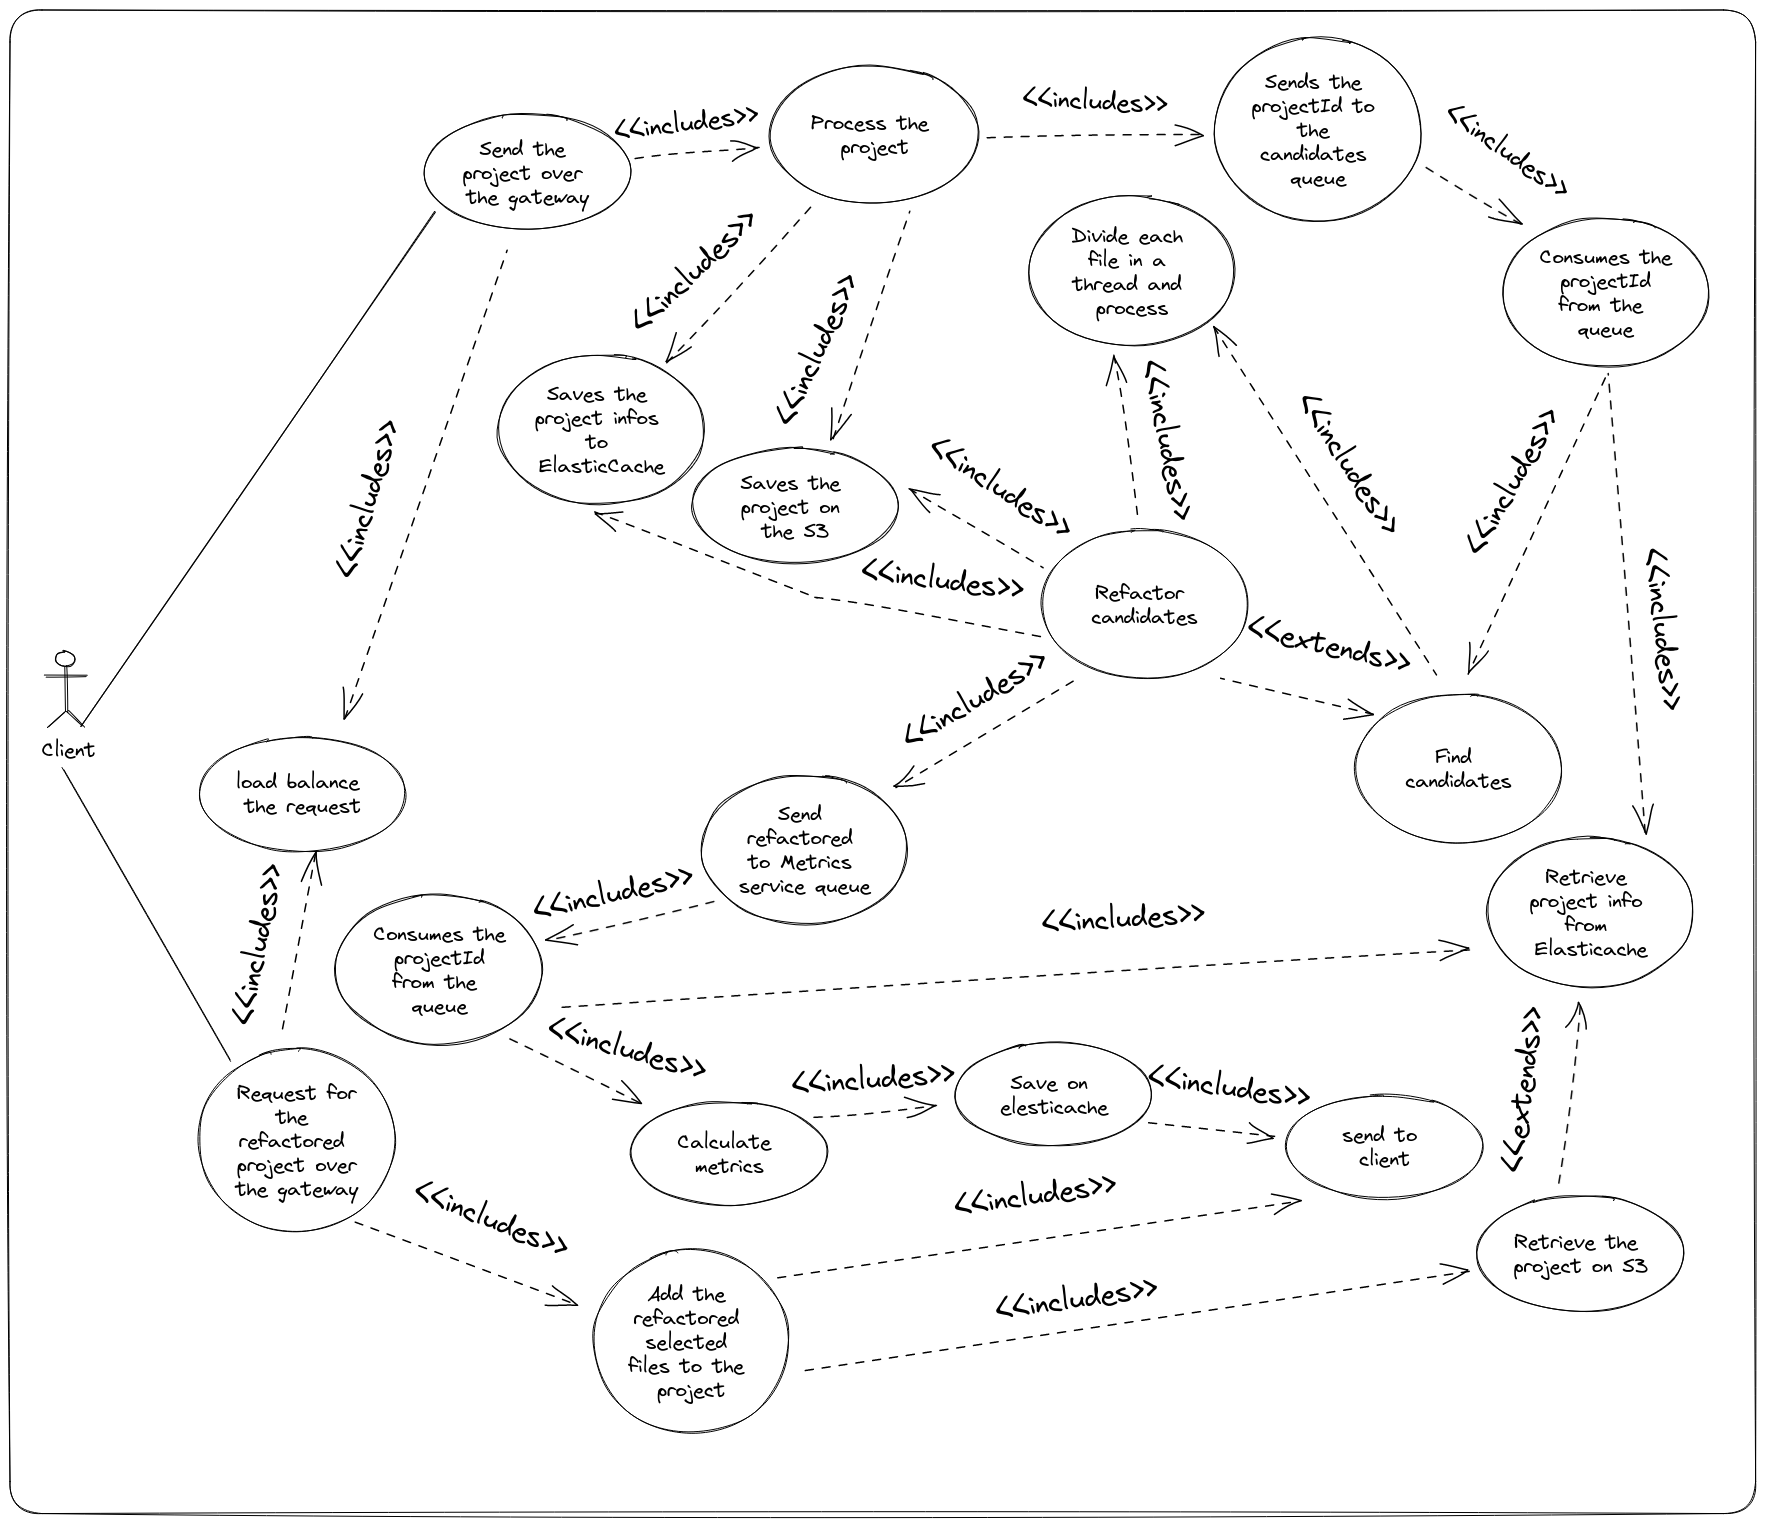
\includegraphics[width =\textwidth, scale=0.2]{Chapter-4/Figures/usecasenew.png}
\SourceOrNote{Own authorship (2023)}
\end{figure}


The new tool flow will work as described on the \Cref{fig-async}, starting with the user selecting the project and sending it over to the API Gateway that will connect with the Intermediary Service by the ELB; the service will have one queue one for finding refactoring candidates, and then refactor it, both will send the information to the Detection Service which will process and send the information to the Metrics Service if any candidate was found. While the Detection and Metrics service is working, the Intermediary service is pulling on the Redis to see if the process is finished to send back the information to the client, which is a long pull on the intermediary service as shown on use case diagram in \Cref{fig-usecasenew}.


\subsubsection{Detection Method Asynchronous Operation}
\label{sub-async}
As seen before, the throttling is happening on the Detection Service as it does not work with threads and has too much file system access; an asynchronous approach with a controlled file system access approach can solve the problem. Making the tool work with thread will improve its performance as it can process many files simultaneously, as described in \Cref{fig-threading}.

\begin{figure}[ht!]
\SetCaptionWidth{\textwidth}
\caption{RMT multi-thread structure}
\label{fig-threading}

\includegraphics[width =\textwidth, scale=0.2]{Chapter-4/Figures/threadDivision.png}
\SourceOrNote{Own authorship (2023)}
\end{figure}

The Detection Service will access the S3 only once per operation, once to search for candidates and once to refactor to solve the problem of the file system being accessed many times to retrieve the project.

When the Detection services receive a project, it will divide the files over the JVM threads to be individually processed simultaneously and compile together after increasing the CPU usage of the service in exchange for performance. The async architecture will help to achieve more threads as it will not hold any thread connection with BFF.

\subsection{Tests implementantion}
\label{sub-tests}

As refactoring is a good practice for coding tests also are. For that reason, unit tests will be applied to the tool for every file with logic, trying to achieve a unit test coverage of 98\% with the help JUnit 5 test framework for Java and Mockito, another Java framework focused on mocking classes and methods.

Unit tests are important, but they cannot guarantee that the integration of the classes and logic is working; that is why integration tests will be implemented with Testcontainers. A framework that manipulates Docker containers to run over tests enabling the service to create a local stack of the cloud environment for tests and use, such as it would work on the production running the application locally with the programmed scenarios.

\section{Java Update \& Framework Refactoring}
\label{sec-framework}

The proposed approach intends to upgrade the RMT tool bridging it to a more modern and robust environment. The first improvement is to change the Spring boot framework, a Java framework enterprise-ready and widely used in the market according to \textcite{Mythily2022}. The framework change is supported by three main reasons described below.
\begin{itemize}
\item Java EE 8 works but has some drawbacks compared to new technologies, such as no integrated server, barriers to the developer running the tool, and losing time configuring a web server. On the other hand, Spring has a tomcat web server integrated and only needs one maven command to be ready and running.
\item Spring boot has production-ready cloud-native data, among other integrations, which reduces the programming and configuration time.
\item As the RMT is divided into services, Spring has built-in tools to manage services like the Eureka service registry. Now the management is made by the tool.
\end{itemize}

Following the framework update, an architecture change is also planned, altering the communication of the services to be async so each service would run independently and faster than the current sync architecture. To support all the new features, the infrastructure of the RMT will be based on the AWS cloud service as it provides high scalability and availability, so the user does not have to run the program on his computer.

Following the refactoring proposal, the spring boot framework will be used. The community highly supports it and has many libraries built to help its development.
The first step to upgrade the services is to change the Java version from 8 to 17, which will receive support until 2024. This change was based on new features such as better support for containers, records, and many other improvements after Java 8 release \cite{java8to17}. 

The RMT tool uses Java EE to create injection dependencies, web servers, and many other configurations; since Java 8, the ownership has changed from Oracle to Eclipse foundation, changing its imports from Javax to Jakarta EE described by \textcite{java8to17} on the oracle blog.

The Spring ecosystem will substitute the JavaEE, an open-source framework that uses the Jakarta EE implementations to work but abstracts many functionalities for the programmer. According to the \textcite{javasurvey}, Spring has up to 57\% of the market share compared with other frameworks; it's best to consider that Spring does not compete with Jakarta EE. The change is based on the spring facility to integrate with the cloud, having projects like spring cloud only to facilitate the development of cloud-native applications. These Spring data offer abstractions to communicate to databases, among others.

\section{Closing Remarks}
\label{sec-closingproposal}
The proposal of tool refactoring presented in this chapter focused on addressing several flaws identified in the RMT tool. The proposed changes involved an internal and external architecture that aims to improve the scalability, performance, and accessibility of the tool through the cloud. The RMT tool's communication changes were directed towards creating more configuration over failure, using queues over HTTP requests. 

The proposed infrastructure was deployed on the AWS cloud, and technologies can be used locally with the AWS LocalStack. The new architecture uses Fargate, Amazon SQS, AWS API Gateway, ELB, Elasticache Redis, and S3 Bucket services. 

The RMT tool's database was changed to Amazon S3 and Elasticache, with SQS substituting most of the REST calls of the tools. The Intermediary Service works only as a BFF communicating with the Detection Service. This proposal allows the RMT tool to work asynchronously, with users having to pull information on the BFF, verify the status on the Elasticache, and send information to the client when it is ready.